\subsection{Общий принцип ГА}\label{subsec:ga_general_principles}
Идея работы генетического алгоритма заимствована у природы: также, как в ходе эволюции, происходит появление оптимального организма для заданных условий — в ходе работы алгоритма ищется набор параметров, при котором фитнесс-функция максимальна.

В природе тот, кто лучше приспособлен к окружающей среде, в большей степени получает доступ к размножению,
в результате чего новые особи получают признаки от лучших родителей.
Из-за того, что геном наследуется от обоих родителей, получившиеся комбинации могут по-новому комбинировать в себе черты,
что даёт большое преимущество перед бесполым размножением (аналогом которого являются такие методы оптимизации, как градиентный спуск или отжиг).
Нужно пояснить, что половое размножение не обязательно предполагает наличие нескольких полов.
Особи в ГА — аналоги гермафродитов из живой природы: в отличие от людей, каждая особь может скрещиваться с каждой.

Это позволяет именно лучшим чертам, по каким-либо причинам появившихся у особей, переходить в следующее поколение.

За их появление отвечают мутации — небольшие случайные изменения в геноме.

Из принципа работы можно понять, что алгоритм \href{https://en.wikipedia.org/wiki/Heuristic_(computer_science)}{эвристический}: сложно доказать его сходимость или что-либо гарантировать с вероятностью 100\%.
Зато исследования (\url{talgat.org/news/wp-content/uploads/2018/08/112.pdf}) показывают, что именно этот алгоритм даёт лучшие результаты для самых сложных функций.
В разделе \ref{subsubsec:hazing}, какие меры предпринимаются, чтобы не дать алгоритму попасть в локальный минимум, не добравшись до глобального.

\subsection{Термины}\label{subsec:ga_principles}
Набор параметров представляется в виде \textit{«генома»} — некой структуры данных, содержащей информацию об этом наборе.
\textit{Особь} — в контексте алгоритма будет использоваться в качестве синонима к геному.

Геном состоит из \textit{генов} — каждый из них содержит информацию о каком-либо признаке (в случае природы) или параметре (в случае ГА).

В каждый момент времени алгоритм работает с \textit{популяцией} — набором геномов.
Это аналог популяции в природе.

Мутация — как и в реальной жизни — небольшое случайное изменение генома без строго определённого направления.

\subsection{Примерная последовательность действий ГА}\label{subsec:approx_ga_algo}
В общих чертах работа ГА выглядит так:

\underline{Инициализация}: Сгенерировать случайную популяцию, каждый ген каждого генома — в заданных пределах.

Затем — повторять, пока не закончится заданное количество итераций или не будет достигнуто требуемое значение фитнесс-функции:

\begin{enumerate}
    \item Посчитать фитнесс-функции для каждой из особей.
    Для большинства задач этот шаг занимает бо́льшую часть времени исполнения,
    поэтому нужно оптимизировать именно его, в частности — распараллелить,
    запуская независимые вычисления на нескольких потоках.

    \item Каким-либо образом отобрать особи на скрещивание

    \item Произвести скрещивание, получив «отпрысков» — часть нового поколения

    \item Сформировать новое поколение, используя, возможно, в разных пропорциях, различные источники геномов, а именно:

    \begin{itemize}

        \item Отпрысков, полученных на предыдущем шаге в результате скрещивания
        \item Лучшие особи из прошлой популяции

        \item Случайные особи — чтобы не дать алгоритму сойтись раньше времени, попав в локальный минимум

        \item Возможно, результаты скрещивания одновременно более двух особей.

    \end{itemize}

    \item Произвести мутации в некоторых особях этого поколения (лучшие из мутаций внедрятся в популяцию на следующих итерациях).

    \item Опционально — «обрезать» (то есть насильственно подправить)
    те мутации, которые привели к выходу каких-либо параметров или их комбинаций за пределы допустимого.

    \item Если алгоритм подходит к концу, добавить лучший геном из предыдущего поколения (чтобы он не подвергся мутации)

\end{enumerate}

\subsection{Конкретная реализация ГА и авторские модификации}\label{subsec:my_modifications}

Учитывая тот факт, что в большинстве задач, решаемых мною, бо́льшая часть вычислительного времени ($\gg 95\%$) используется для подсчёта функции ошибки, а не для маниппуляций с геномами
(это подтверждается результатами профайлинга),
задача состоит в том, чтобы минимизировать количество подсчётов функции ошибки, пусть и ценой более долгой работы с геномами.

Первое изменение — отказ от дискретного кодирования геномов.

Для алгоритма по каждой переменной задан её диапазон.

Традиционный подход — разделить диапазон на $2^N$ частей и кодировать номер части в геноме как битовую последовательность из $N$ бит.
Для подсчёта функции ошибки этот номер перекодируется назад в соответствующую точку непрерывной величины.
Мутацией в данном случае является изменение случайного количества каких-то битов этого номера.

А скрещивание обычно происходит путём случайного выбора значений каждого из двоичных разрядов в родительских геномах.

Предварительное тестирование показало бо́льшую эффективность хранения самого числа (без кодирования) по сравнению с традиционным подходом (хранение битовой последовательности), однако планируется провести более тщательное тестирование (см. \ref{itm:testing_system})

\subsection{Операция «скрещивание»}\label{subsec:matting}

Выбор особей для скрещивания происходит пропорционально значению фитнесс-функции в некоторой (небольшой) степени,
что увеличивает разнообразие, так как в случае небольшой степени «оригинальные» геномы, но с неидеальной функцией ошибки могут попасть в «отцы».

Для реализации используется «рулетка» с кумулятивными вероятностями и бинарный поиск по ней при генерации новой особи по случайному числу от 0 до 1.

Само размножение (по умолчанию) осуществляется так: имея два родителя, каждый ген с некоторой вероятностью
либо берётся от отца, либо от матери, либо (так как это непрерывный вещественный параметр)
генерируется по такой плотности вероятности (значения параметра у двух родителей — два крайних максимума на этой кривой):

\begin{figure}[h!]
    \centering
    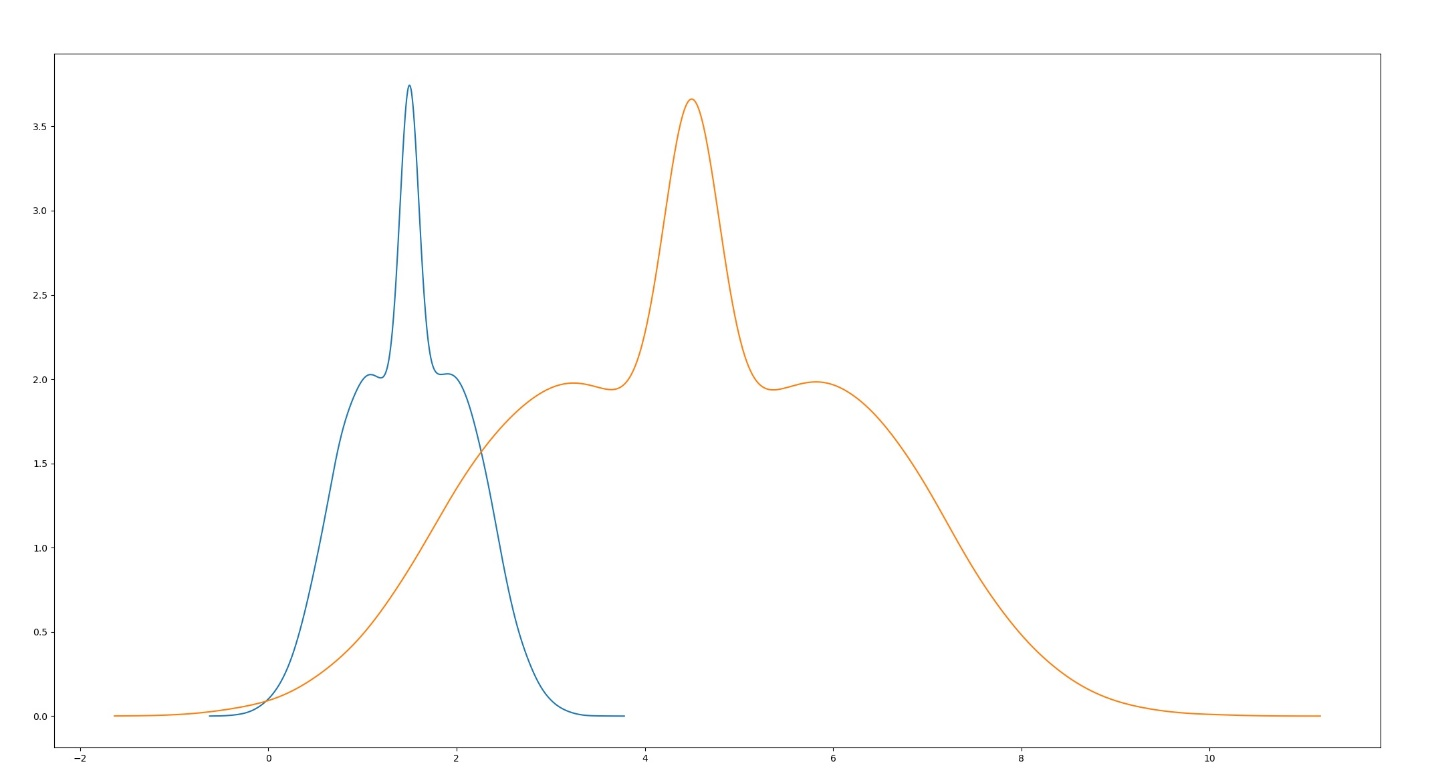
\includegraphics[width=0.75\textwidth]{matting.jpeg}
    \caption{Синяя кривая — для близких геномов, оранжевая — для более далёких}
    \label{fig:}
\end{figure}
\FloatBarrier

Кривая формируется через сумму трёх нормальных распределений.

Она было подобрано таким образом, чтобы наилучшим образом раскрывались
потенциальные возможности генетического материала: максимумы, например, наблюдаются в изначальных точках
и в центре между ними — это именно то, что может нам «дать» такой генетический материал.

Факт в том, что при использовании обычного бинарного кодирования просто-напросто
дискредитируется изначальная природа данных, что не позволяет достичь хороших результатов.

\subsubsection{hazing\_percent: скорость сходимости}\label{subsubsec:hazing}

При использовании алгоритма оптимизации должен поддерживаться баланс
между скоростью сходимости и избежанием застревания в локальном оптимуме.

В случае моей модификации ГА этот баланс регулируется коэффициентом hazing\_percent.

При формировании новой популяции, как было сказано выше, используются разные категории геномов:

\begin{itemize}

    \item Некоторое количество отпрыски, полученные на предыдущем шаге в результате скрещивания (Подробнее про это — в разделе~\ref{subsec:matting}): назовём их $children$.
    \item Иногда — лучшая особь из предыдущей популяции (одна) — $best\_genome$.
    \item Некий набор «элитарных» геномов ($elite$) — отбор на эти места осущевляется пропорционально фитнесс-функции также в некой степени, но уже в большей,
            что делается её действительно элитной.

    \item Гиперэлита ($hyper\_elite$) — то же самое, но меньше мест и больше степень.

    \item … (Остальные)

\end{itemize}

Изменяя распределения мест по категориям, можно регулировать скорость сходимости.
На это распределение и влияет параметр hazing («дедовщина»):
высокое его значение приводит к доминированию уже сформировавшихся геномов и скорейшей их «дошлифовке»,
однако не даёт новым, «подающим надежды» развиться и закрепиться.

Кроме того, в каждой эпохе (итерации) определяется распределение, учитывая процент выполнения алгоритма
— к концу запускается режим максимальной дедовщины: все, кто смог подать надежду, уже закрепились, осталось как раз их «дошлифовать».

(Нужно исследовать всю область поиска,
поэтому нужно не давать сразу огромный бонус при размножении и переходе в другое поколение за некоторое преимущество.)

Только так получится обеспечить развитие нескольких «очагов», внутри которых и будет происходить «шлифование» «идеи искать в этой области».

В будущем планируется сделать распределение мест по степеням отбора непрерывным,
исследовать его, найти оптимальное (возможно — тоже с помощью метаалгоритма оптимизации).


\section{Грядущие улучшения в ГА}\ref{sec:ga-upgrades}

